\documentclass{article}
\usepackage[T1]{fontenc}
\usepackage{titlesec}
\usepackage{graphicx}
\usepackage{amsmath}
\titleformat{\section}  % which section command to format
  {\fontsize{10}{12}\bfseries} % format for whole line
  {\thesection} % how to show number
  {1em} % space between number and text
  {} % formatting for just the text
  [] % formatting for after the text
\title{Logika Cyfrowa}
\author{Jakub Gałaszewski} 
\begin{document}
\maketitle
\section{ Udowodnij używając \textbf{tabeli logicznej}, że $x \vee y \wedge z = (x \vee y) \wedge (x \vee z)$.}
 \textbf{tabela logiczna} to reprezentacja wyrażeń logicznych za pomocą tabelki, gdzie zmienne logiczne przybierają wartość prawdziwą i fałszywą. W tabelce logicznej rozpatrujemy wszystkie kombinacje zmiennych, aby sprawdzić (lub udowodnić) prawdziwość danych stwierdzeń.\\
załóżmy  że $\phi \equiv x \vee y \wedge z = (x \vee y) \wedge (x \vee z)$
W naszym przypadku rozpiszemy wartości każde wartości logiczne dla x, y, z ($2^3$) aby udowodnić podany w zadaniu przykład:\\
\begin{center}
	\begin{tabular}{|c|c|c|c|c|c|c|c|c|} 
	 \hline
	 $x$ & $y$ & $z$ & $x \vee y \wedge z$ & $(x \vee y)$ & $(x \vee z)$ & $(x \vee y) \wedge (x \vee z)$& $\phi$\\ 
	 \hline \hline
	 0 & 0 & 0 & 0 & 0 & 0 & 0 & 1\\ 
	 \hline
	 0 & 0 & 1 & 0 & 0 & 1 & 0 & 1\\ 
	 \hline
	 0 & 1 & 0 & 0 & 1 & 0 & 0 & 1\\ 
	 \hline
	 0 & 1 & 1 & 1 & 1 & 1 & 1 & 1\\ 
	 \hline
	 1 & 0 & 0 & 1 & 1 & 1 & 1 & 1\\ 
	 \hline
	 1 & 0 & 1 & 1 & 1 & 1 & 1 & 1\\ 
	 \hline
	 1 & 1 & 0 & 1 & 1 & 1 & 1 & 1\\ 
	 \hline
	 1 & 1 & 1 & 1 & 1 & 1 & 1 & 1\\ 
	 \hline
	 
	\end{tabular}
\end{center}
czyli $\phi$ jest tautologią.
\section{ Udowodnij używając \textbf{diagramu Venna}, że $x \wedge y \vee y \wedge z \vee \neg x \wedge z = x \wedge y \vee \neg x \wedge z$.}
\textbf{Diagram Venna} to diagram najczęściej przedstawiane w postaci "okręgów", reprezentują one zbiory wartości.
\begin{center}
	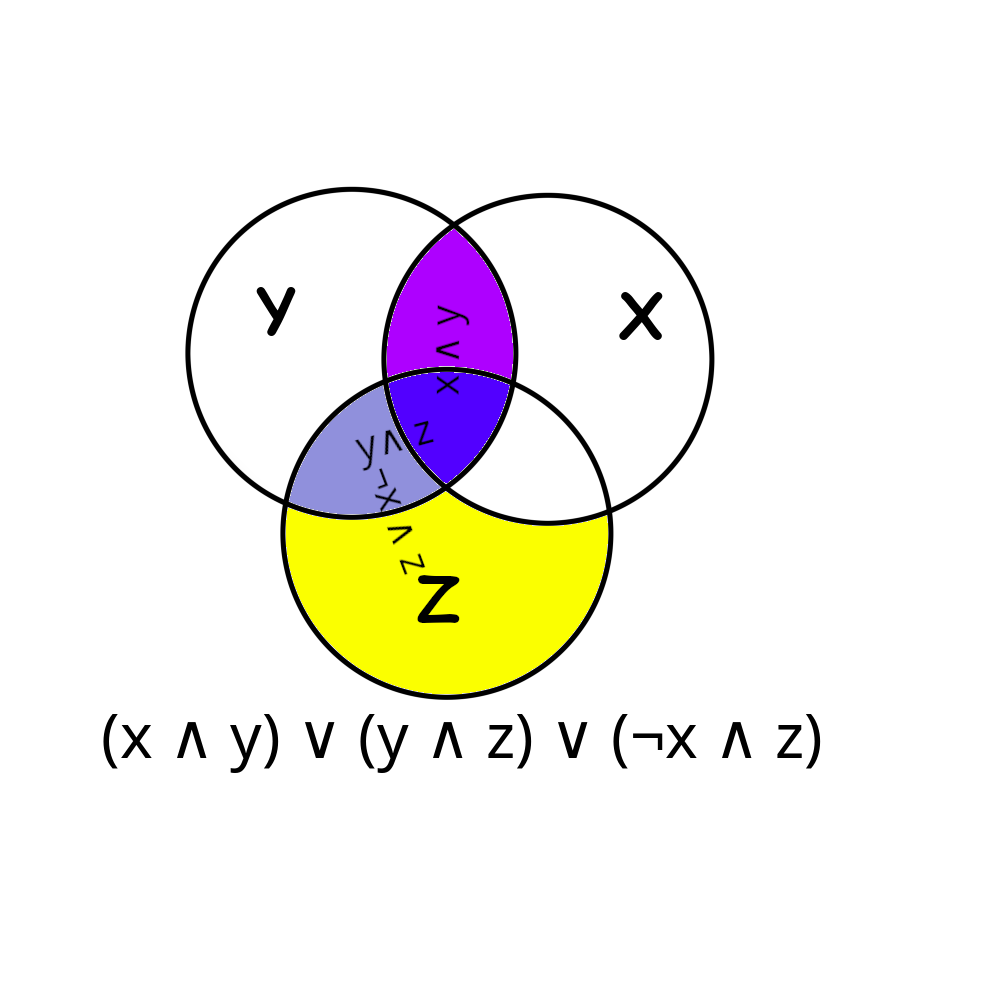
\includegraphics[scale=0.4]{./L01Z02czI.png} $\equiv$ 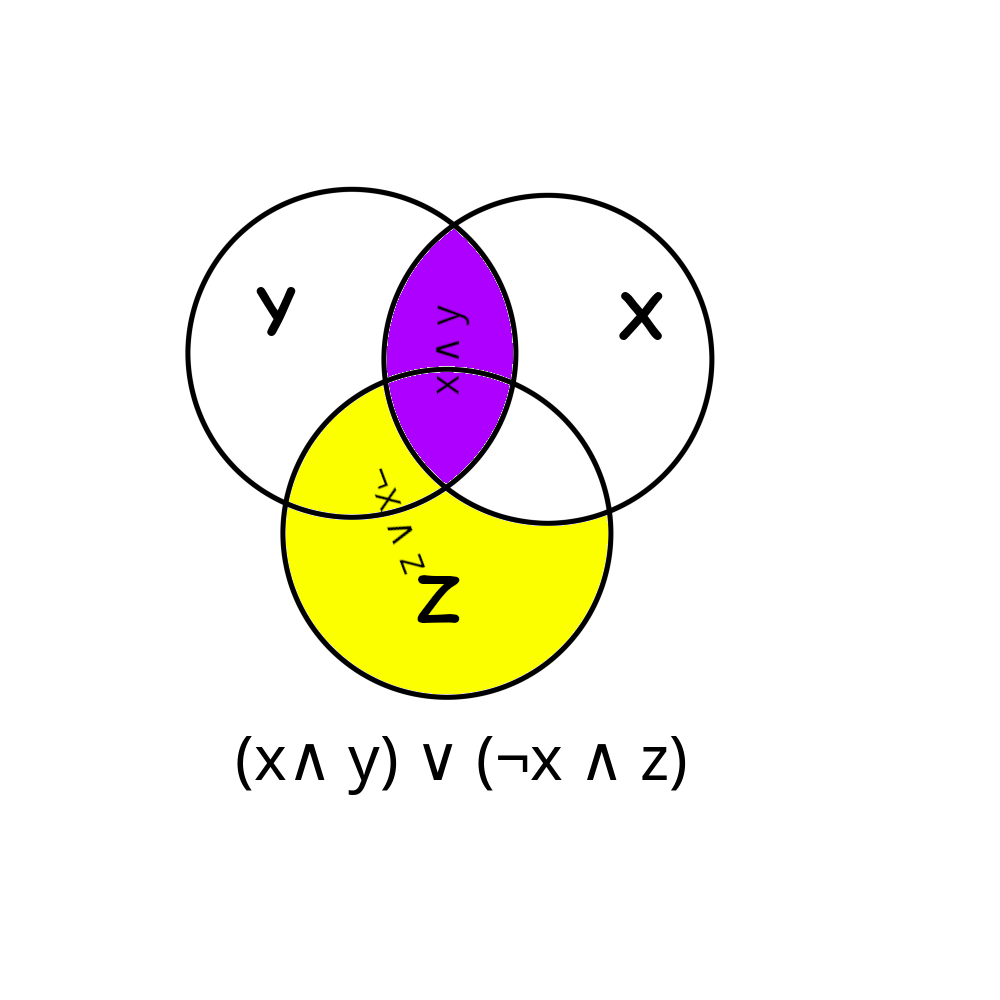
\includegraphics[scale=0.4]{./L01Z02czII.png}
\end{center}
\section{Udowodnij używając diagramu Venna, że $(x \vee y \vee z) \wedge (x \vee y \vee \neg z) = x \vee y$.}
\begin{center}
	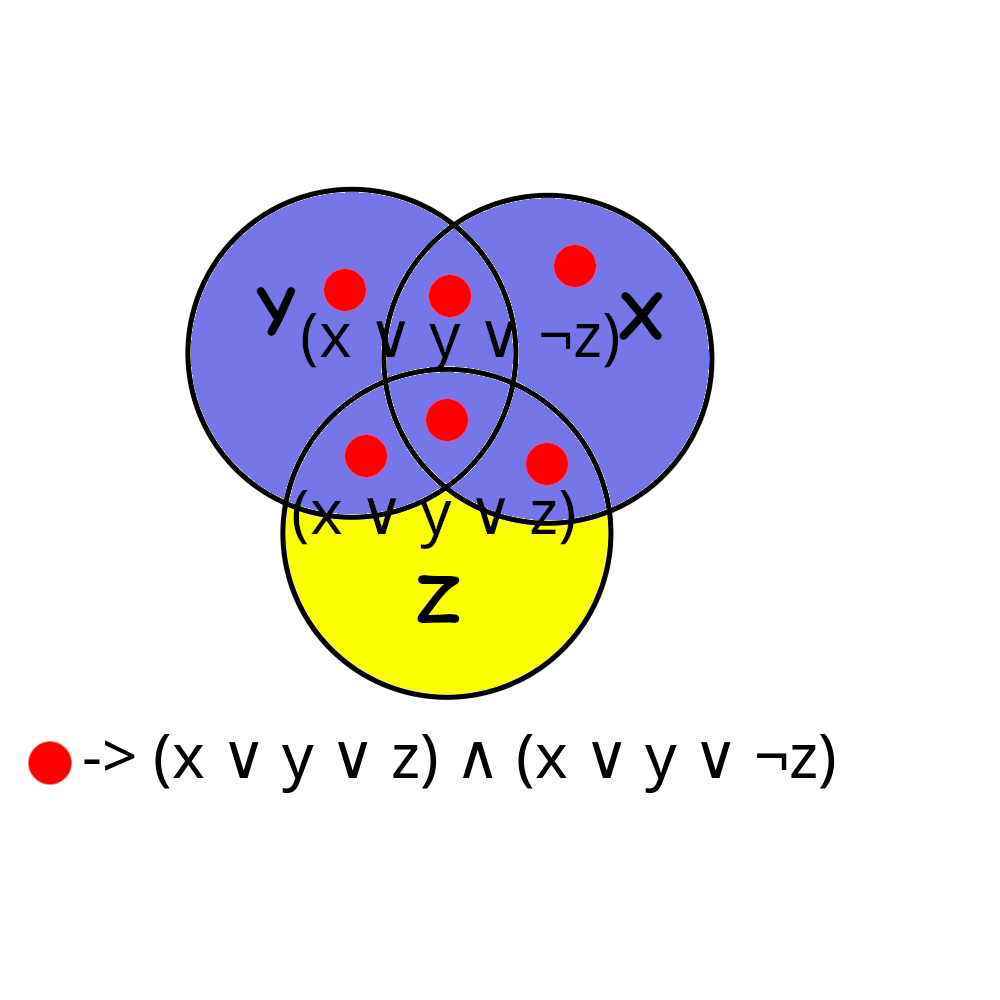
\includegraphics[scale=0.4]{./L01Z03czI.png} $\equiv$ 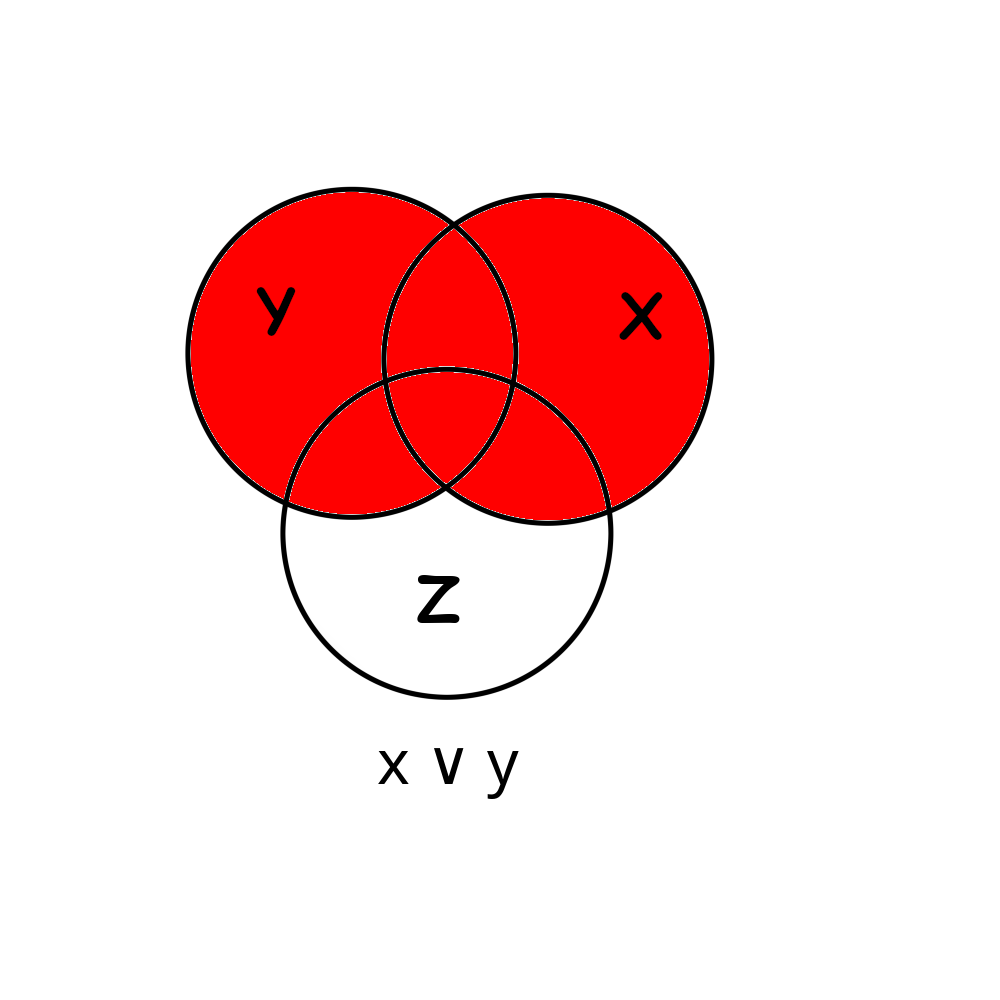
\includegraphics[scale=0.4]{./L01Z03czII.png}\\
\end{center}
\section{Udowodnij przez przekształcenia algebraiczne algebry Boole’a, że $(x \wedge y) \vee (x \wedge \neg y) = x$}
\textbf{Algebra Boole'a} jak nazwa wskazuje to algebra, która składa się z 0, 1, koniunkcji, alternatywy, negacji. Podobnie jak zbiory algebraiczne posiada dla nich charakterystyczne własności, np łączność, przemienność, absorpcja.\\
\begin{gather*}
(x \wedge y) \vee (x \wedge \neg y) =  (x \wedge y \vee x) \wedge (x \wedge y \vee \neg y) = \\ ((x \wedge y) \vee (x \wedge x)) \wedge (x \wedge y \vee \neg y) = \\ x \wedge ((\neg y \vee x) \wedge (\neg y \vee y)) = x \wedge (\neg y \vee x) = \\ (x \wedge \neg y) \vee (x \wedge x) = x \wedge \neg y \vee x = x
\end{gather*}
można też zdecydowanie prościej:
\begin{gather*}
(x \wedge y) \vee (x \wedge \neg y) = x \wedge (y \wedge \neg y) = x \wedge 1 = x
\end{gather*}
\section{Udowodnij przez przekształcenia algebraiczne algebry Boole'a, że $x \wedge y \vee y \wedge z \vee \neg x \wedge z = x \wedge y \vee \neg x \wedge z$. Możesz użyć równości z poprzedniego zadania.}
\begin{gather*}
x \wedge y \vee y \wedge z \vee \neg x \wedge z = \\ 
(x \wedge y) \vee (\neg x \wedge z) \vee (y \wedge z \wedge 1) = \\ 
(x \wedge y) \vee (\neg x \wedge z) \vee (y \wedge z \wedge (x \vee \neg x)) = \\ 
(x \wedge y) \vee (\neg x \wedge z) \vee (y \wedge z \wedge x) \vee (y \wedge z \wedge \neg x)) = \\ 
(x \wedge y) \wedge (1 \vee z) \vee (\neg x \wedge z) \wedge(1 \vee y) = \\
x \wedge y \vee \neg x \wedge z\\
\end{gather*}
\section{Uprość przez przekształcenia algebraiczne algebry Boole’a formułę $\neg x \wedge \neg y \vee \neg x \wedge y \wedge \neg z \vee \neg (x \vee \neg z)$}
\begin{gather*}
\neg x \wedge \neg y \vee \neg x \wedge y \wedge \neg z \vee \neg (x \vee \neg z) = \\ 
 \neg (\neg x \vee y) \vee \neg (x \vee \neg z) \vee (\neg x \wedge y \wedge \neg z) = \\ 
\neg (( x \vee y) \wedge (x \vee \neg z)) \vee (\neg x \wedge y \wedge \neg z) = \\ 
\neg (((x \vee y) \wedge x) \vee ((x \vee y) \wedge \neg z)) \vee (\neg x \wedge y \wedge \neg z) = \\
\neg (x \vee (x \vee y) \wedge \neg z) \vee (\neg x \wedge y \wedge \neg z) = \\
(\neg x \wedge \neg (x \vee y) \vee z) \vee (\neg x \wedge y \wedge \neg z) = \\
(\neg x \wedge \neg x \wedge \neg y \vee z) \vee (\neg x \wedge y \wedge \neg z) = \\
 (\neg x \wedge \neg y \vee z) \vee (\neg x \wedge y \wedge \neg z) = \\ 
 \neg x((\neg y \vee z) \vee (y \wedge \neg z)) =   \neg x(\neg(y \wedge \neg z) \vee (y \wedge \neg z)) =\\ \neg x \wedge 1 = \neg x
\end{gather*}
\section{Napisz możliwie prostą formułę algebry Boole’a odpowiadającą poniższej tabelce oraz narysuj możliwie
prosty układ logiczny realizujący tę formułę:}
\begin{center}
\begin{tabular}{|c|c|c|c|} 
	 \hline
	 $x$ & $y$ & $z$ & $f(x, y, z)$\\ 
	 \hline \hline
	 0 & 0 & 0 & 0 \\ 
	 \hline
	 0 & 0 & 1 & 1\\ 
	 \hline
	 0 & 1 & 0 & 1\\
	 \hline
	 0 & 1 & 1 & 1\\ 
	 \hline
	 1 & 0 & 0 & 1\\ 
	 \hline
	 1 & 0 & 1 & 1\\ 
	 \hline
	 1 & 1 & 0 & 1\\ 
	 \hline
	 1 & 1 & 1 & 0\\ 
	 \hline
\end{tabular}

\end{center}
\textbf{układ logiczny} to Diagram, w którym do każdego wejścia bramki jest podłączone co najwyżej jedno wyjście (być może innej bramki). Reprezentuje się w sposób wizualny.\\
korzystając z wiedzy o DNF i CNF łatwo można wyznaczyć formułę, która jest postaci $(x \vee y \vee z) \wedge \neg (x \wedge y \wedge z)$\\
A układ logiczny wygląda następująco:
\begin{center}
	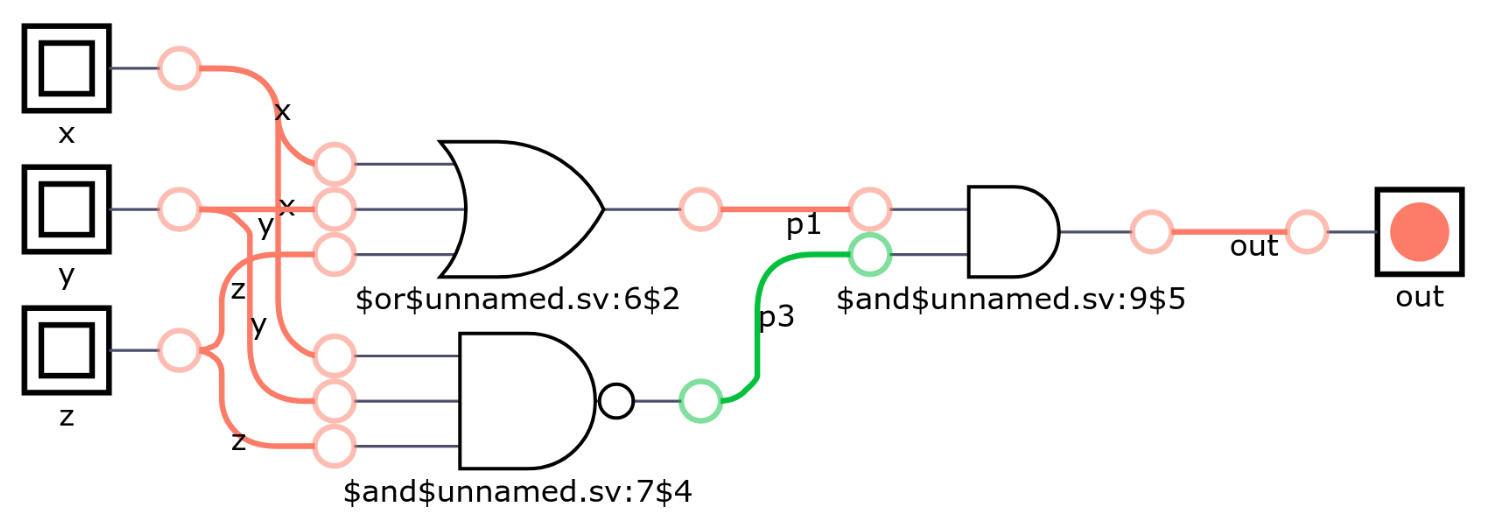
\includegraphics[scale=0.2]{./L01Z07.png}
\end{center}
\section{Uprość poniższy układ logiczny używając praw de Morgana. Zapisz formułę algebry Boole’a odpowiadającą
uproszczonemu układowi.}
\begin{center}
	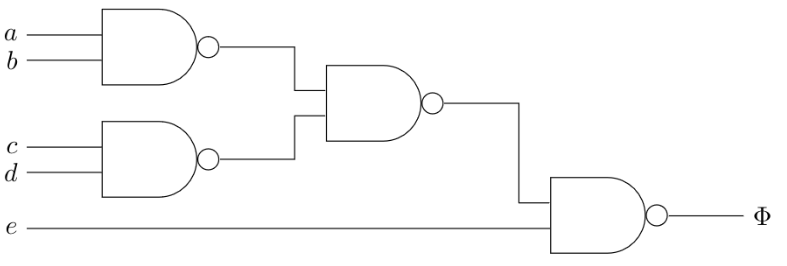
\includegraphics[scale=0.4]{./L01Z08.png}
\end{center}
Powyższy układ logiczny można przedstawić w następujący sposób:
$$\neg(\neg(\neg(a \wedge b) \wedge \neg(c \wedge d))\wedge e)$$\\
w zależności od zrozumienia treści, możemy przekształcić albo "zrzucając" negację do zmiennych, lub  ograniczając liczbę negacji. 
\begin{gather*}
\neg(\neg(\neg(a \wedge b) \wedge \neg(c \wedge d))\wedge e) = \\ \neg(((a \wedge b) \vee (c \wedge d))\wedge e)
\end{gather*}
powyższe przekształcenie ogranicza do minimum liczbę bramek logicznych:
\begin{center}
	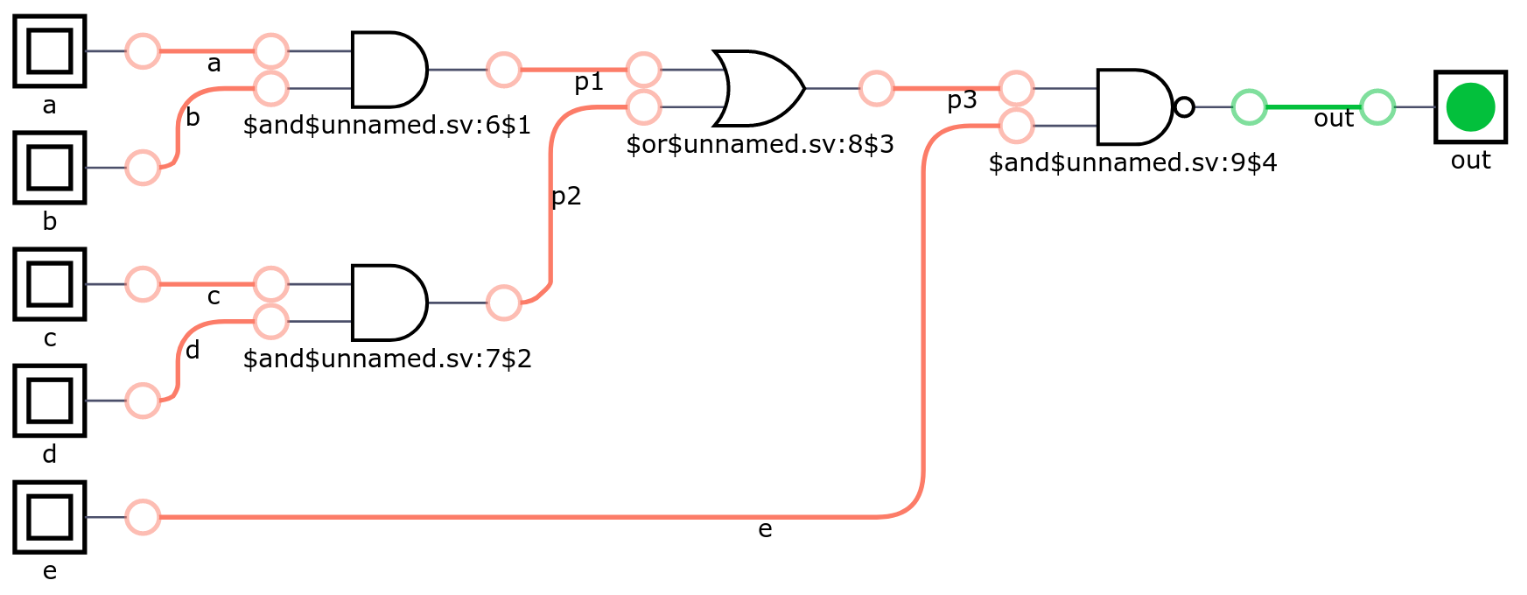
\includegraphics[scale=0.2]{./L01Z08LC.png}
\end{center}
Całość można uprościć jeszcze bardziej, ale układ logiczny będzie bardziej zaawansowany:
\begin{gather*}
\neg(\neg(\neg(a \wedge b) \wedge \neg(c \wedge d))\wedge e) = \\ \neg(a \wedge b) \wedge \neg(c \wedge d)\vee \neg e = \\ (\neg a \vee \neg b) \wedge (\neg c \vee \neg d)\vee \neg e
\end{gather*}
\section{Narysuj układ logiczny, który zawiera cykl, ale pomimo tego reprezentuje pewną funkcję logiczną. Narysuj
układ bez cyklu reprezentujący tę samą funkcję.}
\begin{center}
	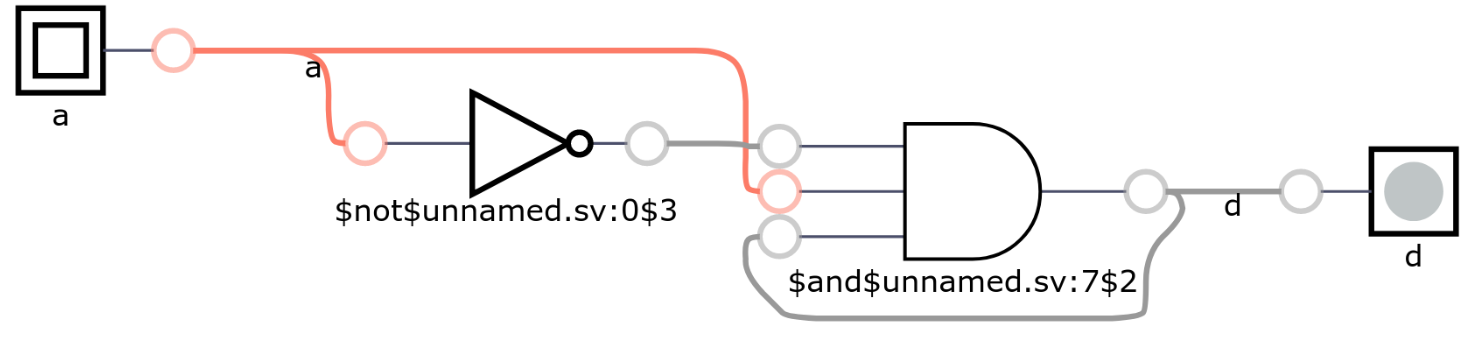
\includegraphics[scale=0.2]{./L01Z09.png}
	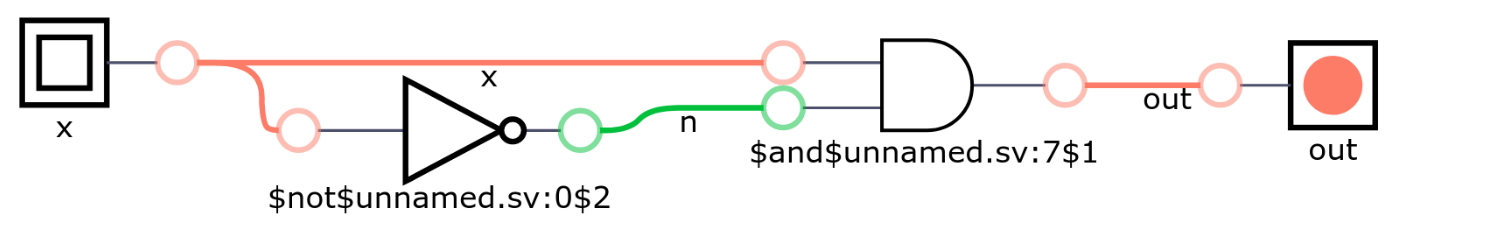
\includegraphics[scale=0.3]{./L01Z09czII.png}
\end{center}
 \end{document}